\documentclass[11pt]{article}

\usepackage{fontspec}
\usepackage{polyglossia}
\setmainlanguage{greek}
\setotherlanguage{english}
\setmainfont{DejaVu Serif}
\setsansfont{DejaVu Sans}
\setmonofont{DejaVu Sans Mono}[Scale=0.85]

\usepackage{graphicx}
\usepackage{geometry}
\geometry{a4paper, margin=2.4cm}
\usepackage{amsmath}
\usepackage{amssymb}
\usepackage{booktabs}
\usepackage{array}
\usepackage{multirow}
\usepackage{xcolor}
\definecolor{ntuablue}{HTML}{0B3D6B}
\definecolor{ntuagray}{HTML}{4A4A4A}
\usepackage[colorlinks=true, linkcolor=ntuablue, urlcolor=ntuablue]{hyperref}

\newcommand{\code}[1]{\texttt{\small #1}}
\newcommand{\en}[1]{\textenglish{#1}}

\setlength{\parskip}{0.45em}

\begin{document}

\begin{titlepage}
\centering
\sffamily

\vspace*{0.5em}

\includegraphics[width=0.20\textwidth]{ntua-logo.png}\\[1.4em]
{\large\bfseries\color{ntuablue} Εθνικό Μετσόβιο Πολυτεχνείο}\\[0.5em]
{\normalsize\color{ntuagray} Σχολή Ηλεκτρολόγων Μηχανικών και Μηχανικών Υπολογιστών}\\[0.3em]
{\normalsize\color{ntuagray} Δ.Π.Μ.Σ. «Επιστήμη Δεδομένων και Μηχανική Μάθηση»}

\vfill

{\color{ntuablue}\rule{\linewidth}{1.5pt}}\\[1.4em]
{\LARGE\bfseries\color{ntuablue} Διαχείριση Δεδομένων\\[0.3em] Μεγάλης Κλίμακας}\\[1.2em]
{\large\color{ntuagray} Εξαμηνιαία εργασία}\\[1.4em]
{\color{ntuablue}\rule{\linewidth}{1.5pt}}

\vfill

{\renewcommand{\arraystretch}{1.3}
\begin{tabular}{@{}r@{\hskip 1.2em}l@{}}
{\bfseries\color{ntuablue} Φοιτητής}             & Γεώργιος Σκουρτσίδης \\
{\bfseries\color{ntuablue} Α.Μ.}                 & 03400314 \\[0.9em]
{\bfseries\color{ntuablue} Διδάσκοντες}          & Δημήτριος Τσουμάκος \\
                                                 & Ιωάννης Κωνσταντίνου \\[0.4em]
{\bfseries\color{ntuablue} Υπεύθυνος εργαστηρίου} & Νικόλαος Χαλβατζής \\
\end{tabular}}

\vspace{2.5em}

{\large\color{ntuagray} Ακαδημαϊκό έτος 2025--2026}
\vspace{1em}

\end{titlepage}

\section{Περιβάλλον και εκτέλεση}

Η εργασία υλοποιήθηκε σε \en{Java} 17 και εκτελείται πάνω σε \en{Spark} 3.5.8 και
\en{Hadoop} 3.4.1, στο \en{Kubernetes} cluster του εργαστηρίου. 
Η υποβολή γίνεται με χρήση ενός βοηθητικού script (\code{submit.sh})
σε \en{cluster mode}. O driver και οι \en{executors} δημιουργούνται ως εφήμερα
\en{pods} από την εικόνα \code{apache/spark:3.5.8-java17}.

Η προεπιλεγμένη εικόνα του \en{Spark} χρησιμοποιεί \en{Java} 11, οπότε δηλώνεται
ρητά το αντίστοιχο \code{java17} tag.

Κάθε \en{query} χωρίζεται σε μια συνάρτηση
\code{compute()} με τη λογική και ένα μικρό \code{main} που φορτώνει τα δεδομένα,
χρονομετρά και τυπώνει. Αυτό γίνεται για λόγους testability: με χρήση τοπικών \en{unit tests},
ελέγχουμε την ορθότητα χωρίς καν να χρειάζεται cluster.

\paragraph{Αποθετήριο κώδικα (code repository)} \url{https://github.com/SkourtsidisGiorgos/ntua-bigdata-2026}

\section{Aνάλυση δεδομένων}

Πριν την υλοποίηση έγινε μια πρώτη εξέταση των δεδομένων (EDA) με χρήση \en{jupyter notebook}.
Τα δεδομένα αποθηκεύτηκαν τοπικά από το \en{remote HDFS} και στη συνέχεια διαβάστηκαν με \en{pandas} και \en{geopandas}.

Παρατηρήσεις:

\begin{itemize}
\item \textbf{\en{Crime data}} (609\,MB και 288\,MB, 28 στήλες, \en{CSV} με
εισαγωγικά): τα δύο αρχεία ενώνονται. Η ημερομηνία δίνεται σε μορφή
\code{2010 Feb 20 12:00:00 AM} και η ώρα ως ακέραιος \en{HHMM}. Η τιμή \code{STREET}
ανήκει στη στήλη \code{Premis Desc}. Στις συντεταγμένες υπάρχουν αρκετές εγγραφές
(0,0), που αντιστοιχούν σε άγνωστη θέση και απορρίπτονται στο \en{Query}~4.
\item \textbf{\en{Census blocks}} (\en{GeoJSON}, $\sim$172\,MB): ένα \en{Feature}
ανά γραμμή. Με \code{multiLine=true} ολόκληρο το αρχείο διαβαζόταν ως ένα
\en{record} και προκαλούσε \en{OOM} στους \en{executors}. Επιλέχθηκε ανάγνωση
γραμμή προς γραμμή, κατανεμημένη και χαμηλή σε μνήμη. Διατηρούνται \code{ZCTA20},
\code{POP20}, \code{HOUSING20}.
\item \textbf{\en{Income}} (\en{CSV} με «;», 282 γραμμές): το εισόδημα δίνεται σε
μορφή «\$52,806», τα σύμβολα αφαιρούνται και η τιμή μετατρέπεται σε ακέραιο. Δύο
\en{zip} δεν έχουν εισόδημα.
\item \textbf{\en{Police stations}} (21 γραμμές): η κεφαλίδα φέρει \en{BOM}, οπότε
οι στήλες λαμβάνονται κατά θέση. Το \code{X} αντιστοιχεί στο γεωγραφικό μήκος και
το \code{Y} στο πλάτος.
\end{itemize}

Πέρα από την \en{EDA} στο \en{notebook}, γράφτηκαν \en{tests} που διαβάζουν τα
πραγματικά αρχεία και επαληθεύουν τα μεγέθη (282 γραμμές με 2 κενές τιμές, 21
σταθμοί, περίπου 300 \en{zip}).

Ακολουθεί ένα παράδειγμα από το EDA: η κατανομή των εγκλημάτων ανά ώρα της ημέρας
(Σχήμα~\ref{fig:hours}). Η εγκληματικότητα είναι χαμηλότερη τις πρώτες πρωινές ώρες
(04:00--05:00) και αυξάνεται προς το βράδυ.

\begin{figure}[h]\centering
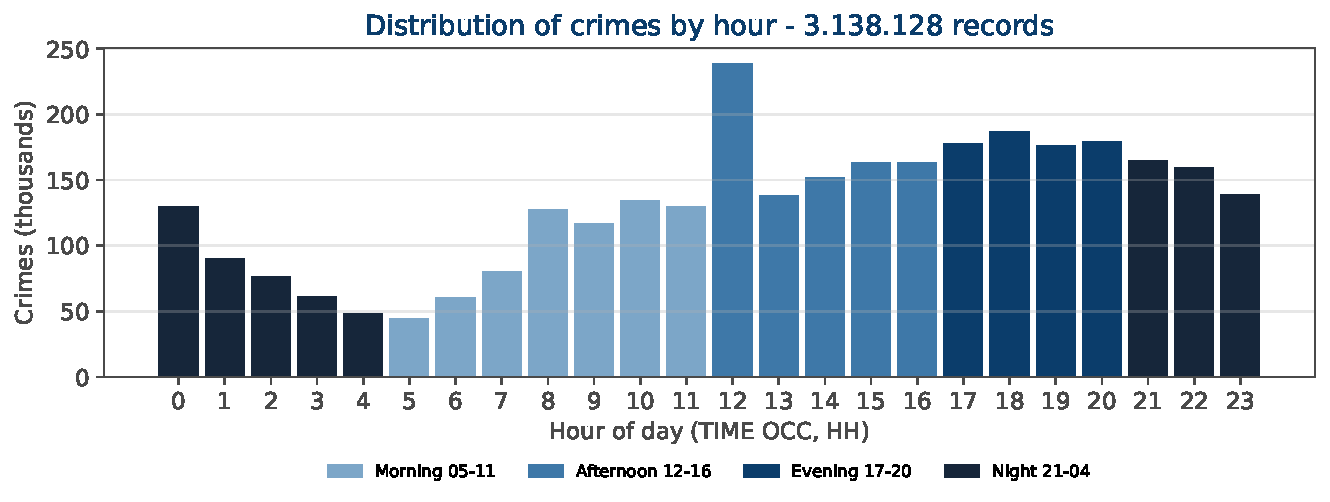
\includegraphics[width=\linewidth]{fig_crime_hours.pdf}
\caption{\footnotesize Κατανομή των εγκλημάτων ανά ώρα, χρωματισμένη κατά τμήμα ημέρας
(όρια \en{Query}~1). Η κορυφή στις 12:00 είναι \en{artifact}, όπου οι άγνωστες ή μη καταγεγραμμένες ώρες
αποθηκεύονται ως μεσημέρι}
\label{fig:hours}
\end{figure}

\section{Mορφή αποθήκευσης}

Τα δεδομένα δίνονται σε \en{CSV}. Τα \en{CSV} είναι αρχεία κειμένου χωρίς σχήμα,
δεν έχει συμπίεση και είναι \en{row oriented}, οπότε το \en{Spark} διαβάζει και να αναλύει όλες τις στήλες κάθε γραμμής.

Υπάρχουν καταλληλότερες μορφές για αναλυτικά φορτία. Το \en{Parquet} και το \en{ORC}
είναι \en{columnar}, δηλαδή αποθηκεύουν τα δεδομένα κατά στήλη, οπότε ένα ερώτημα διαβάζει
μόνο όσες στήλες χρειάζεται (\en{column pruning}). Η αποθήκευση κατά στήλη δίνει και
καλύτερη συμπίεση, καθώς οι τιμές κάθε στήλης είναι ομοιογενείς, ενώ τα στατιστικά
ανά \en{block} (max, min, count) επιτρέπουν να παρακάμπτονται ολόκληρα
\en{blocks} χωρίς ανάγνωση (\en{predicate pushdown}). Το \en{Avro} είναι αντίθετα
\en{row based}, διαθέτει όμως σχήμα και δυαδική, συμπαγή αναπαράσταση, και ταιριάζει
καλύτερα σε σενάρια εγγραφής ή ροής με εξέλιξη σχήματος (\en{schema evolution}). Τα
\en{Parquet} και \en{ORC} είναι παρόμοια στην λειτουργία τους. Επιλέχθηκε το \en{Parquet},
καθώς αποτελεί την προεπιλεγμένη \en{columnar} μορφή στο \en{Spark}, και έχει καλή συμπίεση και υψηλή απόδοση.%
\footnote{Πηγές: τεκμηρίωση \en{Apache Parquet}
(\url{https://parquet.apache.org/docs/}) και \en{Apache Spark SQL: Data Sources}
(\url{https://spark.apache.org/docs/latest/sql-data-sources.html}), επίσης
B.~Chambers \& M.~Zaharia, \emph{Spark: The Definitive Guide}, O'Reilly, 2018, κεφ.~9.}

Για τη σύγκριση, τα δεδομένα \en{crime} μετατράπηκαν σε \en{Parquet} και το ίδιο
\en{Query}~2 εκτελέστηκε και στις δύο μορφές, με 4 \en{executors}.

\begin{table}[h]\centering
\begin{tabular}{lrr}
\toprule
Μορφή (\en{Query}~2, 4$\times$1\en{c}/2\en{GB}) & Χρόνος (ms) & Μέγεθος στο \en{HDFS} \\
\midrule
\en{CSV}     & 57.825 & $\sim$897\,MB \\
\en{Parquet} & 6.524  & 140\,MB \\
\bottomrule
\end{tabular}
\caption{Επίδραση της μορφής αποθήκευσης. Η εφάπαξ μετατροπή κόστισε 89.787\,ms.}
\label{tab:format}
\end{table}

Η διαφορά είναι περίπου εννεαπλάσια, με ταυτόχρονη μείωση του μεγέθους κατά έξι
φορές.
Το \en{Query}~2 χρειάζεται μόνο τις στήλες \code{year} και \code{month}, οπότε από
τις 28 στήλες οι 26 αγνοούνται. Αυτό εξηγεί γιατί το \en{Parquet} είναι
$\sim$140\,MB έναντι 897\,MB του \en{CSV} και ο χρόνος έπεσε από 57.825 σε
6.524\,ms. Το κέρδος προέρχεται και από το \en{column pruning} και από την απουσία
του κόστους \en{parsing} του \en{CSV}. Η μετατροπή έχει κόστος περίπου 90
δευτερόλεπτα.

\section{Query 1 (DataFrame, UDF, RDD)}

Ζητείται η κατάταξη των τμημάτων της ημέρας με βάση το ποσοστό των εγκλημάτων που
σημειώθηκαν στον δρόμο. Τα όρια είναι: Πρωί 05:00 ως 11:59,
Απόγευμα 12:00 ως 16:59, Βράδυ 17:00 ως 20:59, Νύχτα 21:00 ως 04:59. Ο παρονομαστής
(σύνολο εγγραφών) είναι κοινός για όλα τα τμήματα, επομένως δεν επηρεάζει την
κατάταξη. Το ποσοστό δίνεται επί του συνόλου των εγγραφών με έγκυρη ώρα
(3.138.128 εγγραφές). Και οι τρεις υλοποιήσεις παράγουν παρεμφερή αποτέλεσμα:

\begin{table}[h]\centering
\begin{tabular}{lrr}
\toprule
Τμήμα ημέρας & Εγκλήματα \en{STREET} & Ποσοστό (\%) \\
\midrule
Νύχτα (\en{Night})       & 251.094 & 8{,}0014 \\
Βράδυ (\en{Evening})     & 198.292 & 6{,}3188 \\
Απόγευμα (\en{Afternoon})& 156.432 & 4{,}9849 \\
Πρωί (\en{Morning})      & 130.866 & 4{,}1702 \\
\bottomrule
\end{tabular}
\caption{Query 1: ποσοστό εγκλημάτων \en{STREET} ανά τμήμα ημέρας.}
\end{table}

\begin{table}[h]\centering
\begin{tabular}{lr}
\toprule
Υλοποίηση (2 \en{exec} $\times$ 1\en{c}/2\en{GB}) & Χρόνος (ms) \\
\midrule
\en{DataFrame}        & 46.966 \\
\en{DataFrame + UDF}  & 43.163 \\
\en{RDD}              & 28.055 \\
\bottomrule
\end{tabular}
\caption{Query 1: χρόνοι εκτέλεσης.}
\end{table}

Περιμέναμε να υπερτερεί το \en{DataFrame}. Αντ' αυτού, η \en{RDD} υλοποίηση ήταν 
ταχύτερη. Το αποτέλεσμα πιθανόν οφείλεται στο ότι το query είναι ελαφρύ.
Ενα φιλτράρισμα και μια συγκέντρωση σε τέσσερα κλειδιά, χωρίς βαρύ
\en{shuffle}. Η \en{RDD} διαβάζει μόνο δύο στήλες και εκτελεί \code{reduceByKey} με
τοπική σύνθεση (\en{map-side combine}), χωρίς το επιπλέον κόστος του πλάνου. Το
\en{UDF} παρουσίασε ουσιαστικά τον ίδιο χρόνο με το καθαρό \en{DataFrame}. Το \en{UDF} αποτελεί \en{black box} για τον \en{Catalyst} και δεν συμμετέχει στο
\en{whole-stage codegen}, αλλά εδώ η κατηγοριοποίηση της ώρας είναι αρκετά
φθηνή ώστε η διαφορά να ειναι αμελητέα.

\section{Query 2 (DataFrame και SQL)}

Για κάθε έτος ζητούνται οι 3 μήνες με τα περισσότερα εγκλήματα και η θέση τους στην
κατάταξη. Χρησιμοποιείται \code{ROW\_NUMBER} σε παράθυρο ανά έτος, με \en{tie-break}
στον μήνα ώστε το \en{top-3} να είναι ντετερμινιστικό. Οι δύο υλοποιήσεις δίνουν
ταυτόσημο αποτέλεσμα, 48 γραμμές. Για το 2010, για παράδειγμα, προκύπτουν οι μήνες
1, 3 και 7.

\begin{table}[h]\centering
\begin{tabular}{lr}
\toprule
Υλοποίηση (4 \en{exec} $\times$ 1\en{c}/2\en{GB}) & Χρόνος (ms) \\
\midrule
\en{DataFrame} & 57.825 \\
\en{SQL}       & 35.234 \\
\bottomrule
\end{tabular}
\caption{Query 2: χρόνοι εκτέλεσης.}
\end{table}

Η διαφορά στους χρόνους δεν θεωρείται σημαντική. Και οι δύο διατυπώσεις περνούν από
τον ίδιο \en{Catalyst} και καταλήγουν στο ίδιο φυσικό πλάνο, οπότε αναμένονται
παρόμοιοι χρόνοι. Το μεγαλύτερο κόστος είναι το διάβασμα του \en{CSV} και το
\en{shuffle} της \code{GROUP BY}. Έγιναν πολλά τρεξίματα που έδωσαν διαφορετικούς χρόνους, 
γεγονός που αποδίδεται στον φόρτο του κοινόχρηστου cluster. Το τελευταίο ενισχύεται από το
γεγονός ότι τα πειράματα έτρεξαν την τελευταία ημέρα της προθεσμίας
και προσωπική εκτίμηση είναι ότι πολλοί φοιτητές έτρεξαν τα queries τους την ίδια ημέρα.

\section{Query 3 (DataFrame και RDD)}

Ζητείται το μέσο κατά κεφαλήν εισόδημα ανά \en{zip} για την περίοδο 2020-2021. Το
διαθέσιμο εισόδημα που μας δίνεται το dataset είναι ανά νοικοκυριό και όχι ανά άτομο. Έγινε μετατροπη σε κατά
κεφαλήν, διαιρώντας με το μέσο μέγεθος νοικοκυριού, το οποίο προκύπτει από το
\en{census}:
\[
\text{κατά κεφαλήν} = \frac{\text{εισόδημα νοικοκυριού}}{\text{πληθυσμός}/\text{νοικοκυριά}}
= \text{εισόδημα} \cdot \frac{\text{νοικοκυριά}}{\text{πληθυσμός}}.
\]
Τα νοικοκυριά προσεγγίζονται από το \code{HOUSING20} και το \en{join} γίνεται στο
\en{zip}. Οι δύο υλοποιήσεις συμφωνούν (280 \en{zip}). Στις υψηλότερες θέσεις
εμφανίζονται περιοχές όπως Malibu, Playa Vista και Pacific Palisades. Με αναζήτηση στο google επιβεβαιώθηκε πως πρόκειται για ακριβές
περιοχές, κάτι που αποτελεί ένδειξη ορθότητας του υπολογισμού.

\begin{table}[h]\centering
\begin{tabular}{lr}
\toprule
Υλοποίηση (3 \en{exec} $\times$ 1\en{c}/2\en{GB}) & Χρόνος (ms) \\
\midrule
\en{DataFrame} (αυτόματα \en{BroadcastHashJoin}) & 9.885 \\
\en{RDD} (\code{join} = \en{hash join}) & 17.208 \\
\bottomrule
\end{tabular}
\caption{Query 3: χρόνοι εκτέλεσης.}
\label{tab:q3time}
\end{table}

Εδώ το \en{DataFrame} είναι ξεκάθαρα καλύτερο, αντίστροφα από το \en{Query}~1. Ο
\en{Catalyst} αναγνωρίζει ότι η πλευρά του εισοδήματος είναι μικρή και επιλέγει
\en{BroadcastHashJoin}, την εκπέμπει δηλαδή χωρίς \en{shuffle}. Η \en{RDD}
\code{join} δεν διαθέτει αντίστοιχη βελτιστοποίηση και επιβάλλει \en{shuffle} και
στις δύο πλευρές. Όπου υπάρχει \en{join}, το \en{DataFrame} είναι προτιμότερο, ενώ όπου
πρόκειται για απλή συγκέντρωση, η \en{RDD} επαρκεί.

\section{Query 4 και scalability}

Για κάθε σταθμό ζητείται το πλήθος των εγκλημάτων που βρίσκονται πλησιέστερα σε
αυτόν παρά σε οποιονδήποτε άλλον, καθώς και η μέση απόσταση. Πρόκειται ουσιαστικά
για πρόβλημα πλησιέστερου γείτονα: κάθε έγκλημα συγκρίνεται με τους 21 σταθμούς. Η
υλοποίηση χρησιμοποιεί \en{cross join}. Επειδή η πλευρά των σταθμών είναι ελάχιστη,
ο \en{Spark} επιλέγει \en{BroadcastNestedLoopJoin} και τα εγκλήματα δεν μετακινούνται
για το \en{join}. Στη συνέχεια, ανά έγκλημα κρατείται ο κοντινότερος σταθμός μέσω
\code{min} πάνω σε \code{struct(απόσταση, σταθμός)} και ακολουθεί συγκέντρωση ανά
σταθμό. Η απόσταση \en{haversine} υλοποιήθηκε ως έκφραση στήλης και όχι ως \en{UDF},
ώστε να παραμένει εντός του \en{codegen}, καθώς αποτιμάται περίπου 63 εκατομμύρια
φορές. Πρώτο εμφανίζεται το \en{HOLLYWOOD} με 225.515 εγκλήματα και μέση απόσταση
2,077\,km.

Κατά την κλιμάκωση εμφανίστηκε πρόβλημα με τη μνήμη. Στη μικρότερη
διαμόρφωση (1 πυρήνας, 2\,GB) η εκτέλεση ολοκληρωνόταν κανονικά, ενώ με 2 πυρήνες
ανά \en{executor} οι \en{executors} τερματίζονταν με \en{OOM}. Το πρόβλημα αυτό αρχηκά φαινόταν ανορθόδοξο, καθώς η διαθέσιμη μνήμη ήταν περισσότερη. 
Η αιτία εντοπίστηκε στην \emph{off-heap} μνήμη. Με περισσότερους πυρήνες εκτελούνται ταυτόχρονα
\en{tasks} που γεμίζουν τα \en{buffers} του \en{shuffle} πάνω από το προεπιλεγμένο
\code{memoryOverhead}, οπότε το \en{Kubernetes} τερμάτιζε το \en{pod}. Το πρόβλημα
αντιμετωπίστηκε με αύξηση του \code{memoryOverhead}, που είναι ανεξάρτητο από τη
\en{heap} μνήμη της εκφώνησης. Σημειώνεται επίσης ότι η πρώτη εκτέλεση κάθε σειράς
ήταν πιο αργή λόγω \en{cold start} και ότι, λόγω του κοινόχρηστου
cluster, οι μετρήσεις έδιναν διαφορετικούς χρόνους.

\begin{table}[h]\centering
\begin{tabular}{llrr}
\toprule
& Διαμόρφωση & Σύν. \en{cores} & Χρόνος (ms) \\
\midrule
\multirow{3}{*}{Α}
 & 2 \en{exec} $\times$ 1\en{c} / 2\en{GB}  & 2 & 74.162 \\
 & 2 \en{exec} $\times$ 2\en{c} / 4\en{GB}  & 4 & 63.700 \\
 & 2 \en{exec} $\times$ 4\en{c} / 8\en{GB}  & 8 & 65.669 \\
\midrule
\multirow{3}{*}{Β}
 & 2 \en{exec} $\times$ 4\en{c} / 8\en{GB}  & 8 & 65.669 \\
 & 4 \en{exec} $\times$ 2\en{c} / 4\en{GB}  & 8 & \textbf{36.223} \\
 & 8 \en{exec} $\times$ 1\en{c} / 2\en{GB}  & 8 & 204.331 \\
\bottomrule
\end{tabular}
\caption{Query 4: κλιμακωσιμότητα. Πάνω κάθετη (Α), κάτω οριζόντια (Β).}
\label{tab:scal}
\end{table}

\begin{figure}[h]\centering
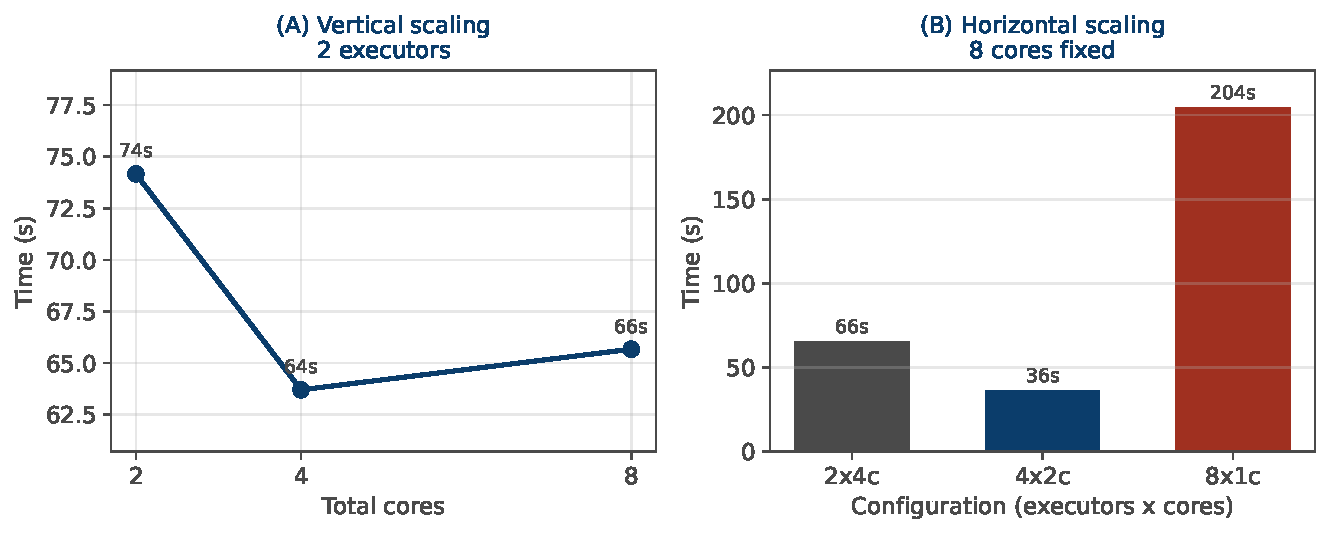
\includegraphics[width=\linewidth]{fig_scalability.pdf}
\caption{\footnotesize Query 4: κλιμακωσιμότητα. (Α) Κάθετη: από 4 πυρήνες και μετά ο χρόνος
σταθεροποιείται (\en{shuffle-bound}). (Β) Οριζόντια με σταθερά 8 \en{cores}: η
ενδιάμεση διαμόρφωση 4$\times$2\en{c} είναι ταχύτερη, ενώ οι 8 μικροί
\en{executors} του ενός πυρήνα είναι ο χειρότερος συνδυασμός.}
\label{fig:scal}
\end{figure}

Στην κάθετη κλιμάκωση (Α), η μετάβαση από 2 σε 4 πυρήνες μείωσε τον χρόνο, ενώ από
4 σε 8 η βελτίωση ήταν αμελητέα. Το ερώτημα δεν περιορίζεται από τη \en{CPU} αλλά
από το \en{shuffle}: το \code{groupBy} ανά έγκλημα είναι το ακριβό στάδιο. Από ένα σημείο και ύστερα οι επιπλέον πυρήνες παραμένουν αναξιοποίητοι. 
Στην οριζόντια κλιμάκωση (Β), με σταθερά τα 8 \en{cores}, ταχύτερη ήταν η διαμόρφωση 4
\en{executors} των 2 πυρήνων. Το τρέξιμο με 2 \en{executors} των 4 πυρήνων ήταν πιο
αργό, ενώ με 8 \en{executors} του ενός πυρήνα ήταν ο χειρότερος συνδυασμός, με 204 δευτερόλεπτα. 
Πολλοί μικροί \en{executors}
συνεπάγονται περισσότερο \en{shuffle} στο δίκτυο και λιγότερη μνήμη ανά
\en{executor}, άρα περισσότερο \en{spill}. Συνολικά, μια ενδιάμεση διαμόρφωση με
λίγους \en{executors} των δύο πυρήνων αποδίδει καλύτερα από τα δύο άκρα.

\section{Στρατηγικές join}

Με χρήση των \code{hint} και \code{explain} εξετάστηκαν οι στρατηγικές \en{join}
που επιλέγει ο \en{Catalyst}.

Στο \en{Query}~3 υπάρχει κλειδί ισότητας (το \en{zip}), οπότε ισχύουν και οι τρεις
βασικές στρατηγικές. Με κάθε \en{hint}, το \code{explain} επιβεβαιώνει τον
αντίστοιχο τελεστή:

\begin{table}[h]\centering
\begin{tabular}{llr}
\toprule
\en{Hint} & Φυσικό \en{join} (από \code{explain}) & Χρόνος (ms) \\
\midrule
\en{BROADCAST}              & \en{BroadcastHashJoin} & 13.516 \\
\en{MERGE}                  & \en{SortMergeJoin}     & 21.245 \\
\en{SHUFFLE\_HASH}          & \en{ShuffledHashJoin}  & 16.172 \\
\en{SHUFFLE\_REPLICATE\_NL} & \en{CartesianProduct}  & 12.814 \\
\bottomrule
\end{tabular}
\caption{Query 3: επίδραση στρατηγικής join (3 \en{exec} $\times$ 1\en{c}/2\en{GB}).}
\end{table}

Οι τρεις από τις τέσσερις στρατηγικές δεν διαφέρουν σημαντικά, με εξαίρεση το
\en{SORT-MERGE}. Πριν το \en{join}, το
\en{census} έχει ήδη συγκεντρωθεί ανά \en{zip}, από 91 χιλιάδες \en{blocks} σε
περίπου 300 γραμμές. Συνεπώς και οι δύο πλευρές του \en{join} είναι πλέον μικρές
και το πραγματικό κόστος βρίσκεται αλλού, στο διάβασμα του \en{GeoJSON}. Το
\en{SORT-MERGE} ήταν παρ' όλα αυτά σταθερά το πιο αργό, καθώς ταξινομεί χωρίς λόγο
και τις δύο πλευρές. Ο αυτόματος χρόνος του Πίνακα~\ref{tab:q3time}, 9.885\,ms,
προέρχεται από προγενέστερη εκτέλεση, γι' αυτό το ρητό \en{BROADCAST} εδώ μετρήθηκε 
ελαφρώς υψηλότερα, πρόκειται για διακύμανση.

Στο \en{Query}~4 δεν υπάρχει κλειδί ισότητας, πρόκειται για \en{cross join}, οπότε
νόημα έχουν μόνο οι \en{nested-loop} στρατηγικές. Αυτό επιβεβαιώθηκε και πειραματικά:
με \en{hint} \en{MERGE}, ο \en{Catalyst} το αγνόησε και επέστρεψε σε
\en{BroadcastNestedLoopJoin}.

\begin{table}[h]\centering
\begin{tabular}{llr}
\toprule
\en{Hint} & Φυσικό \en{join} (από \code{explain}) & Χρόνος (ms) \\
\midrule
\en{BROADCAST}              & \en{BroadcastNestedLoopJoin}, \en{Cross} & 74.162 \\
\en{SHUFFLE\_REPLICATE\_NL} & \en{CartesianProduct}                    & 70.346 \\
\bottomrule
\end{tabular}
\caption{Query 4: επίδραση στρατηγικής join (2 \en{exec} $\times$ 1\en{c}/2\en{GB}).}
\end{table}

Οι δύο χρόνοι σχεδόν ταυτίζονται, όπως αναμενόταν. Δεδομένου ότι οι 21 σταθμοί είναι
αμελητέοι σε μέγεθος, ο μηχανισμός του \en{join} δεν έχει σημασία. Tο κόστος
εστιάζεται στα 63 εκατομμύρια ζεύγη και στο \en{shuffle} που ακολουθεί.

Συνολικά, και στα δύο ερωτήματα η μικρή πλευρά χωράει στη μνήμη, οπότε το
\en{broadcast} είναι η καλύτερη επιλογή: η μικρή πλευρά εκπέμπεται παντού και
αποφεύγεται πλήρως το ακριβό \en{shuffle} της μεγάλης. Το \en{sort-merge} και το
\en{shuffle-hash} αξίζουν μόνο όταν είναι μεγάλες και οι δύο πλευρές, ενώ το
\en{shuffle-replicate-nl} αποτελεί την τελευταία λύση για \en{non-equi join}, και την
ακριβότερη.

\section{Συμπεράσματα}

Το πιο σημαντικό εύρημα αφορά τη μορφή αποθήκευσης. Απλώς μετατρέποντας τα δεδομένα σε
\en{Parquet} επιτάχυνε το \en{Query}~2 σχεδόν εννέα φορές, χωρίς καμία άλλη αλλαγή. 
Ως προς τα \en{API} του \en{Spark}, δεν υπάρχει μία καθολικά σωστή επιλογή. Στο  \en{Query}~1 
ήταν καλύτερη η \en{RDD} υλοποίηση, στο \en{join} του \en{Query}~3
ήταν ταχύτερο το \en{DataFrame}, ενώ \en{SQL} και \en{DataFrame} είναι ισοδύναμα.

Ένα ακόμη σημαντικό συμπέρασμα είναι ότι η αύξηση των πόρων δεν συνεπάγεται απαραίτητα αύξηση στην απόδοση.
Ένα ερώτημα που περιορίζεται από το \en{shuffle}, όπως το \en{Query}~4, παύει κάποια στιγμή να
επιταχύνεται και επιδεινώνεται όταν οι ίδιοι πόροι κατανέμονται σε πολλούς μικρούς \en{executors}.

\end{document}
